% COMMENT THIS OUT TO HIDE SOLUTIONS
\def\SHOWSOLUTIONS{}

\documentclass[12pt]{article}

\usepackage[hidelinks]{hyperref}
\usepackage{comment}
\usepackage{color,graphicx,amsthm,amssymb,amsmath,cite,xspace,setspace}
\usepackage[small,bf]{caption}
\usepackage{multicol,multirow}
\usepackage{algorithm,algorithmic}
\usepackage{soul}
\usepackage{colortbl}
\usepackage{rotating}
\usepackage{textcomp}
\usepackage{epsf}
\usepackage{wasysym}
\usepackage{mdwtab}
\usepackage{bm}
\usepackage{verbatimbox}
\usepackage{framed} % To be able to frame theorems and stuff
\usepackage[most]{tcolorbox}

\usepackage{tikz}
\usepackage{pgfplots}
\pgfplotsset{compat=1.17}


\usepackage{listings}
\definecolor{dkgreen}{rgb}{0,0.6,0}
\definecolor{gray}{rgb}{0.5,0.5,0.5}
\definecolor{mauve}{rgb}{0.58,0,0.82}

\lstset{frame=single,
	aboveskip=3mm,
	belowskip=3mm,
	basicstyle={\ttfamily},
	keywordstyle=\color{blue},
	commentstyle=\color{dkgreen},
	stringstyle=\color{mauve},
	tabsize=3
}


% solutions
\newenvironment{solution}{\vspace{2mm}\color{blue}\textbf{Solution: }}{\color{black}}
\ifdefined\SHOWSOLUTIONS\else\excludecomment{solution}\fi

% define the type of list to use
\usepackage[shortlabels]{enumitem}
\setlist[enumerate,1]{\bfseries 1., itemsep=6mm}
\setlist[enumerate,2]{\bfseries a), itemsep=3mm}

\def\wl{\par \vspace{\baselineskip}} 
\def \bx{\boldsymbol{x}}
\def \bw{\boldsymbol{w}}
\def \bnu{\boldsymbol{\nu}}
\def \by{\boldsymbol{y}}
\def \bz{\boldsymbol{z}}
\def \bu{\boldsymbol{u}}
\def \bv{\boldsymbol{v}}
\def \bb{\boldsymbol{b}}
\def \bg{\boldsymbol{g}}
\def \ba{\boldsymbol{a}}
\def \be{\boldsymbol{e}}
\def \bA{\boldsymbol{A}}
\def\bU{\boldsymbol{U}}
\def \bB{\boldsymbol{B}}
\def \bC{\boldsymbol{C}}
\def \bX{\boldsymbol{X}}
\def \bT{\boldsymbol{T}}
\def \bP{\boldsymbol{P}}
\def \bV{\boldsymbol{V}}
\def \bE{\boldsymbol{E}}
\def \bS{\boldsymbol{S}}
\def \bSigma{\boldsymbol{\Sigma}}
\def \bI{\boldsymbol{I}}

\def\R{{\mathbb R}}
\def\E{{\mathbb E}}
\def\P{{\mathbb P}}
\def \X{{\cal X}}
\def \Y{{\cal Y}}

\DeclareMathOperator{\rank}{rank}
\DeclareMathOperator{\Sign}{sign}
 

\usepackage{fullpage}

% Header and footer
\usepackage{fancyhdr,lastpage}
\pagestyle{fancy}
\cfoot{\thepage\ of \pageref{LastPage}}
\renewcommand{\headrulewidth}{0.0pt}
\renewcommand{\footrulewidth}{0.0pt}

\begin{document}
\begin{center}
{\large ECE 330: Signals \& Systems  -  Applied Homework: Mass Spring Damper System}
\mbox{ }\\
\mbox{ }\\
\end{center}



%\noindent \emph{Note: Please include the names of all the classmates with whom you have collaborated on this activity in your submission.} 

\begin{enumerate}[\qquad 1)]

    \item 
   % \section{Introduction}

The mass-spring-damper system is a classical mechanical model used to describe the dynamic behavior of many physical systems. It consists of three primary components: a mass that represents an object with inertia, a spring that provides a restoring force proportional to displacement according to Hooke's Law, and a damper that introduces resistance proportional to velocity often modeling friction or air resistance.

This system is widely used in engineering and physics to study oscillatory motion, vibrations, and control system dynamics. The mathematical model is typically represented as a second-order differential equation derived from Newtons second law of motion (You will do this soon!). Depending on the damping and external forces, the system may exhibit different types of responses—underdamped, overdamped, or critically damped—making it a useful framework for analyzing and designing mechanical and electrical analog systems (RLC circuits).

\begin{figure}[htbp]
    \centering
    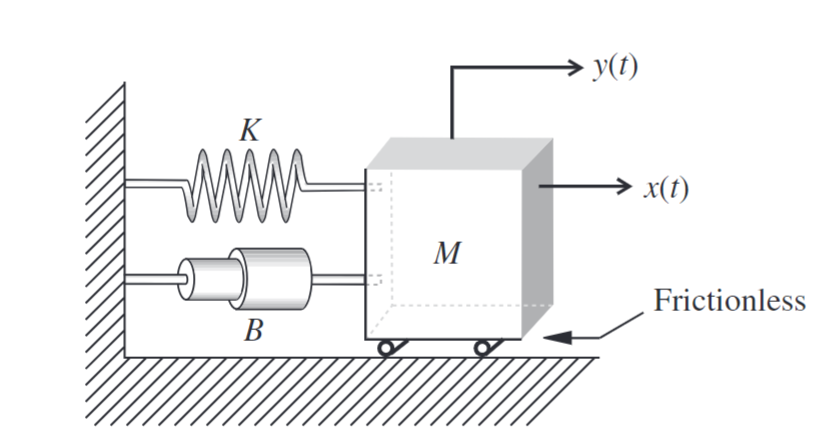
\includegraphics[width=0.5\textwidth]{images/msd_figure.png}
    \caption{Diagram displaying the mass-spring damper system.}
\end{figure}

%\section{Theory}

In this section, you will derive the differential equation for the MSD system and its solutions. You will also analyze the system using Laplace to formulate a PID controller to control the position of the mass. Then, you will use multiple techniques to decide the gains of the controller to get best response.

%\subsection{Differential Form}

To derive the differential equation, you will begin with $F = ma$, Newton's Second Law, where $F$ is the force on the mass, $m$ is the mass, and $a$ is the acceleration. Remember, the force due to a spring is $F = -kx$, where $k$ is the spring constant and $x$ is the mass displacement. Also, the force of a damper is $F = -bv$, where $b$ is a constant and $v$ is velocity. 

Write the differential equation in standard form (coeffiecent of 1 on the highest order derivative) of the system (Hint: $a$ is the second derivative of $x$ and $v$ is the first derivative of $x$):

    \begin{solution}
        $\frac{d^2}{dt^2}x + \frac{b}{m}\frac{d}{dt}x + \frac{k}{m}x = 0$
    \end{solution}

Now, consider the system with the following input: $\frac{d^2}{dt^2}x + \frac{b}{m}\frac{d}{dt}x + \frac{k}{m}x = 7f$, where $f(t) = 8e^{2t}$. Solve for the steady state response.


    \begin{solution}
        $x_s(t) = 2e^{2t}$
    \end{solution}

    
Next, solve for the roots of the transient response of the differential equation if $m = 1, b = 7, k = 10$.

    \begin{solution}
    $s_1 = -5, s_2 = -2$
    \end{solution}


Finally, solve for the constants and give the final form of the full response if $x(0) = 0, x'(0) = 2$. Remember, $x(t) = x_s(t) + x_t(t)$.

    \begin{solution}
        $c_1 = 2, c_2 = -4$
        \\
        $x(t) = 2e^{-5t} - 4e^{-2t} + 2e^{2t}$
    \end{solution}   


Using MATLAB, upload a plot of $x(t)$ where $20 \leq t \leq 30$ with a step of $0.01$.

\begin{solution}
    \begin{figure}[htbp]
        \centering
        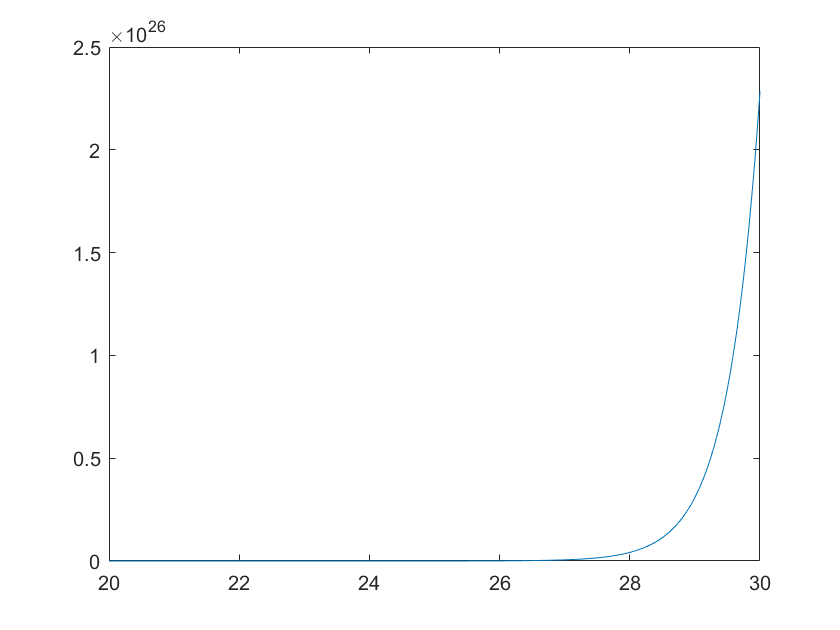
\includegraphics[width=0.3\textwidth]{images/dif_eq_plot.png}
        \caption{Plot of $x(t)$}
    \end{figure}  
\end{solution}


%\subsection{System Root Analysis}

Discuss what the roots do, i.e. damping effects. Have them decide if a couple systems are underdamped, critically damped, or overdamped.

%\subsection{Laplace}

Solve the exact system above using Laplace.

%\section{PID Controller}


%\section{MATLAB Simulation}
		

\end{enumerate}
\end{document}